\chapter{OFFLOADING FRAMEWORK}
\label{chap:offloading}
%
\section{Motivation}
\label{offloading:motivation}
%
Heterogeneity is now the norm in commodity computing systems where
platforms possess a mix of computing units such as CPUs, GPU, and other
specialized accelerators.
%
OpenCL has therefore emerged as the open standard for parallel programming
for these heterogeneous platforms.
%
By providing a common standard along with the necessary toolchain, OpenCL
enables a uniform framework to discover, program, and distribute parallel
workloads to the diverse set of compute units in the hardware.
%
Graphics processing units (GPUs), in particular, have reached the extended
coverage due to their rapidly expanding use in general purpose computing
(GPGPU) with parallel programming of the OpenCL standard.
%
For that reason, there have been efforts exploring the advantages of
parallelism from the OpenCL framework by offloading GPGPU workloads
within an HPC cluster environment~\cite{rcuda,vocl}.
%
The primary motivation for offloading within a cluster is for more efficient
utilization of resources by allowing multiple compute nodes to share the same
GPU for general purpose computing.
%
These researchers clearly demonstrate that OpenCL (and CUDA)-based
remote offloading is a viable option which saves power through more efficient
sharing of heterogeneous compute units over the network despite the
communication overheads.\\
%
In this work, I shift this motivation from the HPC cluster environment
to mobile platforms by considering a different perspective to this
expanding body of research by adapting the OpenCL offloading approach to
a mobile cloud computing scenario.
%
Since previous works focused mainly on offloading OpenCL workloads in
HPC cluster environments with high bandwidth and low latency between the
nodes, it was easy to realize and assess the advantages.
%
However, the advantages are not as clear in the mobile cloud computing
scenario where OpenCL workloads are sent over the wide area on
network links with much lower bandwidth and higher latencies than 
cluster environments.
%
Moreover, since workloads are traversing untrusted networks in the
wide-area, a layer of network encryption is necessary to ensure privacy
and some level of the trust of the results from the remote compute node.\\
%
This section presents an OpenCL-based remote offloading framework designed
specifically for mobile cloud computing where OpenCL workloads can be exported
from a mobile node (i.e. an Android device) to the cloud (i.e.
an Amazon EC2 instance with GPU access).
%
This remote offloading framework consists of the following components:
1) a customized RPC system with optimizations for network tasking and
data marshalling, 2) a service discovery mechanism which selects the 
compute node with the lowest latency, and 3) a virtual private networking 
layer which provides transparent network encryption without any modification 
at the application layer.
%
The proposed system is implemented as a wrapper library around the OpenCL API; thus
allowing transparent integration of the OpenCL API with our framework 
without any code modification.
%
The offloading framework also makes it possible for the developer to 
dynamically discover accelerators located on remote computing nodes 
(i.e. in the cloud), virtualize these accelerators as if they would be
regular accelerators located on-board the local mobile device, and then
seamlessly offload computation to the virtual accelerators.\\
%
An additional contribution of this work is a distributed method of resource management 
which handles service discovery, access control, and data privacy.
%
Past mobile offloading solutions have not investigated a service discovery 
mechanism and they assume the static availability of remote computing nodes 
with fixed endpoints.
%
Instead, this work advocates a dynamic approach where eligible compute nodes are 
discovered at runtime, allowing for a more flexible design. 
%
I achieved this by using IP multicast-based discovery so that the
system periodically locates compute nodes available within their
networks.\\
%
Furthermore, the proposed approach supports accessing resources beyond the local
private network, broadening the accessibility to trusted compute nodes
across the Internet and the cloud.
%
In fact, previous offloading research has focused on sending workloads only to 
resources within private local area networks where there is some guarantee 
that the data is contained within the network.
%
This is accomplished by utilizing a social peer-to-peer virtual 
private network, SocialVPN~\cite{socialvpn}.
%
The use of a peer-to-peer VPN with social features has several benefits.
%
First of all, by providing virtual private IP addresses only to social peers, 
the endpoints discovered through the VPN are deemed trustworthy by the user -– 
creating a Social Area Networks.
%
Secondly, the IP layer security ensures data privacy and frees us from 
having to handle the cumbersome tasks of cryptographic key management, and 
socket layer encryption.
%
Through SocialVPN, the state and functions (called kernels in OpenCL) 
necessary for remote execution are sent privately and the results are 
authenticated and verified at the virtual networking layer.\\
%

\section{The Structure of Remote Offloading Framework}
\label{offloading:structure}
%
The overall architecture of the proposed framework consists of 5 main
modules: integration with the OpenCL API, RPC-based offloading
mechanism, decentralized resource discovery feature, runtime scheduler,
and trusted and private IP communication layer.
%
\begin{figure}
\centering
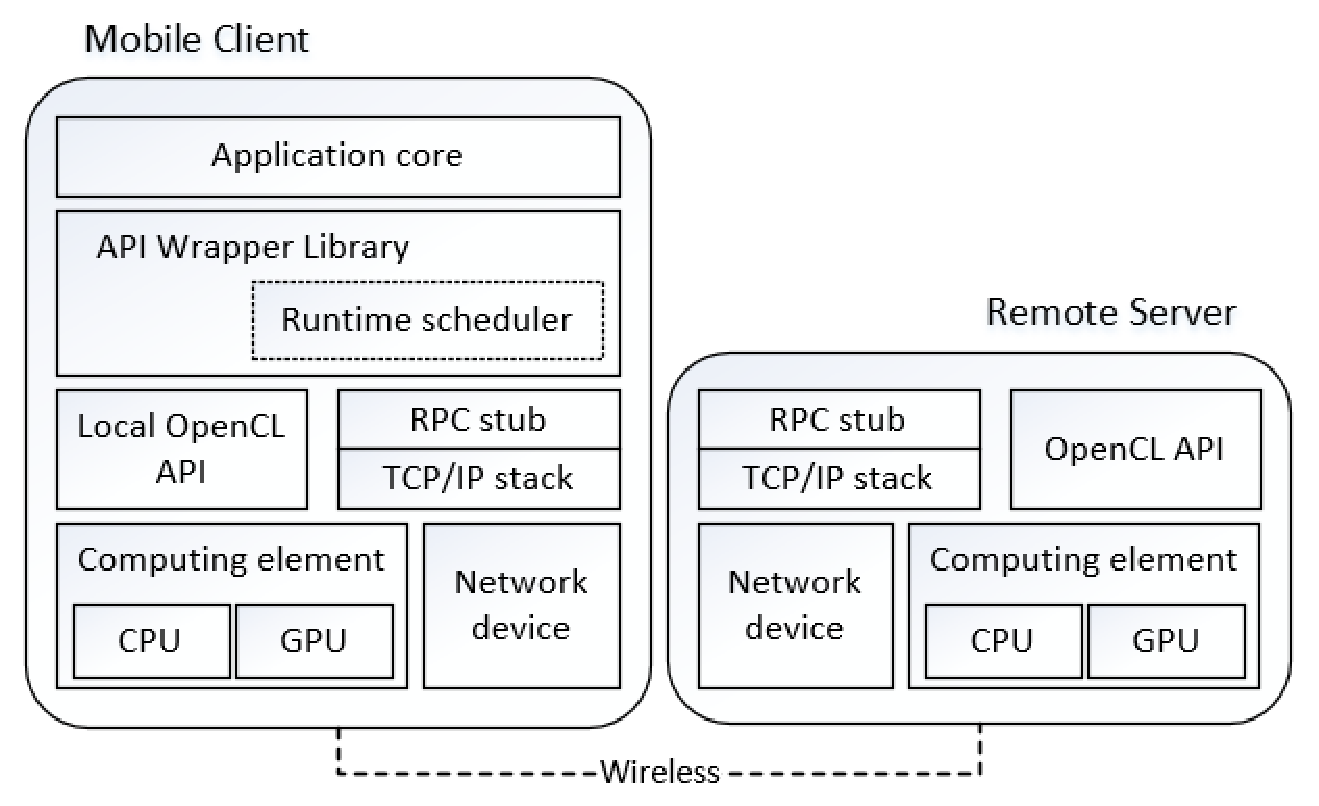
\epsfig{file=figs/overall_arch.eps, width=4.5in}
\caption{Overall system architecture}
\label{fig:architecture}
\end{figure}
%
\subsection{Transparent OpenCL API Extension}
\label{offloading:API}
%
Since OpenCL is an open standard currently supported by most of the
major device manufacturers, I chose not to deviate from their API in
order to minimize the learning curve for developers.
%
Latest revisions of the OpenCL specification are extending the coverage
to enable integration of a large pool of heterogeneous hardware under
the API.
%
Because OpenCL is also a hardware level offloading framework, it
provides various functions which can leverage in the proposed system.
%
The OpenCL API possesses a set of these features: device discovery and
enumeration, device selection and customization, buffer management,
job offload and status queries.
%
With these features, the application developer has a full control on the
use of specific accelerators necessary to optimize their application
performance.
%
In this section, I explain how these features can be extended to support
remote offloading framework.
%
Table~\ref{table:functionality} summaries OpenCL API functionalities and extensions.\\
%
{\bf Device discovery and enumeration.} In the initialization phase of the
interface, the developer queries the platform for on-board
OpenCL-capable accelerators.
%
The OpenCL framework returns a list of accessible compute devices
located on the board along with their computing capabilities (e.g.
graphics cards, video decoders, cryptographic devices).
%
In the case of a mobile device, this might include only a graphics
processor, or a specialized stream processor~\cite{stemcell}.
%
I extend this portion of the API by allowing the developer to discover
other OpenCL-enabled accelerators located on remote computing resources
over the network.
%
Hence, when the developer performs this type of the query on a mobile
device, it discovers not only the local mobile GPU but also another GPUs
running on the remote workstations or on the cloud, as long as they are
part of the same virtual private network.\\
%
{\bf Device selection and configuration.} In the standard OpenCL
framework, once presented with a list of devices, the developer selects
one or more targets for computation offloading.
%
This selection is usually based on the characteristics of each particular
device (e.g. the number of compute units of the accelerator, maximum
number of work items, architecture, latency or network bandwidth).
%
Based on the characteristics the developer is also able to configure the
workload appropriately for better performance.
%
Since this is a hardware layer offloading mechanism, the OpenCL framework
handles the support for different architectures by using a compiler
which converts the code from a modified version of C99 to the target
instruction set of the accelerator.
%
Hence, the API also provides access to compiler-based customizations for
both local and remote devices.
%
By extending the discovery process to include remote OpenCL devices over
the network, this selection and configuration process can become
cumbersome to the developer.
%
Thus, the proposed system can present only one virtual device handle
which represents the best offloading node according to network
conditions.\\
%
{\bf Workload state transfer.} Having selected a device, the next phase 
is the actual offloading of the data and code necessary to run workloads 
remotely.
%
The function to be executed (i.e. a kernel) is first sent either as C99 source
code or an LLVM-based intermediate language.
%
Once transferred, the code is compiled for the target accelerator.
%
In order to execute the kernel on the accelerator, the necessary state has
to be transferred to the device regardless of whether it is local or remote.
%
If the device resides on the host platform, the task of buffer management 
simply involves copying data from main memory to local storage accessible 
by the accelerator.
%
However, if the workload is being offloaded to a remote accelerator, then
the buffers have to be managed slightly differently.
%
First, the data has to be marshalled and copied into the buffers of the
networking stack, then transported over the network to the appropriate
remote host.
%
The data is then copied from the networking stack of the remote host
unto the accelerator's own local storage.
%
For example, in the case of a mobile device offloading computation to a
GPU hosted in the cloud, the necessary input and output buffers have to
be created and copied in the GPU's local memory in the cloud.
%
Upon completion, the output buffers are copied back from the GPU's local
memory to the mobile device's memory over the network.
%
Also, it is possible to perform data compression at the networking layer
to minimize the networking overhead and energy consumption.\\
%
{\bf Resouce and failure management.} The final phase of the OpenCL API
is the ability to discover errors and release its state and resources in
a graceful manner.
%
Each function has its error parameter which keeps the developer aware of
the proper execution of the remote job.
%
If an error occurs due to an issue with the source code, the workload
configuration, or any other hardware issues, an appropriate error code
is returned to the developer.
%
In return, the developer can release the various resources (i.e. buffers,
device handles) that are associated with the job.
%
Once again, I extend this functionality to support network failures as
well.
%
In the case of a disconnection, the appropriate error code is returned
ro the developer who then performs the necessary actions to clean up the
state belonging to the job.
%
On the server, the necessary clean-up is taken as well by the
framework.\\
%
The decision to utilize the OpenCL framework for computation offloading
in mobile devices allows us to leverage all of the functionalities
already in place for offloading computation locally from the CPU to an
on-board hardware accelerator.
%
I added the required extensions to the framework by creating a wrapper
library around the OpenCL API.
%
Since the offloading framework provides an identical interface,
developers can integrate their OpenCL code with the system without any
code modification. 
%
\begin{landscape}
%\begin{sidewaystable}
\begin{table}
	\centering
	\caption{OpenCL API functionalities and extensions}
	
	\begin{tabular}{p{3.0cm}|p{5.5cm}|p{3.5cm}|p{5.0cm}|p{3.7cm}} \hline
    \parbox{3.0cm}{\centering Feature} & \parbox{5.5cm}{\centering API
Function} & \parbox{3.5cm}{\centering OpenCL Feature} &
\parbox{5.0cm}{\centering Extension Capabilities} &
\parbox{3.7cm}{\centering Future Capabilities} \\ \hline

    \parbox{3.0cm}{\centering Discovery and \\Enumeration} & \parbox{5.5cm}{\centering \textit{} \\\textit{clGetPlatformIDs},\\\textit{clGetDeviceIDs},\\\textit{clGetDeviceInfo}
\\\textit{}} & \parbox{3.5cm}{\centering List on-board devices} &
\parbox{5.0cm}{\centering List the best remote resource} &
\parbox{3.7cm}{\centering List all remote resources} \\

    \parbox{3.0cm}{\centering Selection and \\Configuration} &
\parbox{5.5cm}{\centering \textit{}
\\\textit{clCreateContext},\\\textit{clBuildProgram},\\\textit{clCreateKernel},\\\textit{clSetKernelArgs},
\\\textit{clEnqueueNDRangeKernel} \\\textit{}} &
\parbox{3.5cm}{\centering Enables job compilation \\and configuration} &
\parbox{5.0cm}{\centering Configuration for the \\remote resource} &
\parbox{3.7cm}{\centering Configure \\multiple resources} \\

    \parbox{3.0cm}{\centering Workload \\State Transfer} & \parbox{5.5cm}{\centering \textit{}
\\\textit{clCreateProgramWithSource},\\\textit{clCreateBuffer},\\\textit{clEnqueueReadBuffer},\\\textit{clEnqueueWriteBuffer}
\\\textit{}} & \parbox{3.5cm}{\centering Source code and data transfer\\ over the
internal} & \parbox{5.0cm}{\centering Source code and data transfer\\ over
the network} & \parbox{3.7cm}{\centering Explore caching for\\ better performance} \\

    \parbox{3.0cm}{\centering Resource and \\Failure Management} &
\parbox{5.5cm}{\centering \textit{}
\\\textit{clWaitEvents},\\\textit{clFlush},\\\textit{clFinish},\\\textit{clReleaseBuffer},\\\textit{clReleaseProgram}
\\\textit{}}
& \parbox{3.5cm}{\centering Check on status and\\ cleanup} &
\parbox{5.0cm}{\centering Add support for network failure\\ and cleanup} &
\parbox{3.7cm}{\centering Enable timeout for\\ slow responses} \\ \hline
    \end{tabular}
\label{table:functionality}
%\end{sidewaystable}
\end{table}
\end{landscape}
%
\subsection{Integration of OpenCL API with RPC Service}
\label{offloading:rpc}
%
In order to support offloading on the remote resources, the offloading
framework utilizes an RPC-based service which handles offloading
requests received over the virtual private network.
%
As an first attempt, SunRPC service was utilized to provide the remote
procedure calling interface, serialization, and networking capabilities.
%
However, SunRPC provides many extra features that are not necessarily
efficient(for example, the use of a portmapper daemon to discover the
listening port of the RPC service).
%
SunRPC also initiates a new TCP connection for each function call which
incurs extra delay and the overhead on network performance.
%
In contrast, the proposed design uses a single TCP connection per
offloading job thus achieving lower latencies.
%
By running an RPC service which exposes the OpenCL API over the network,
the offloading framework provides a computation offloading design that
is lightweight in terms of argument serialization and buffer management.
%
Other approaches~\cite{vocl} rely on more sophisticated communication
primitives such as MPI which require extra processing and memory
resulting in poor battery performance.\\
%
\begin{figure}
\centering
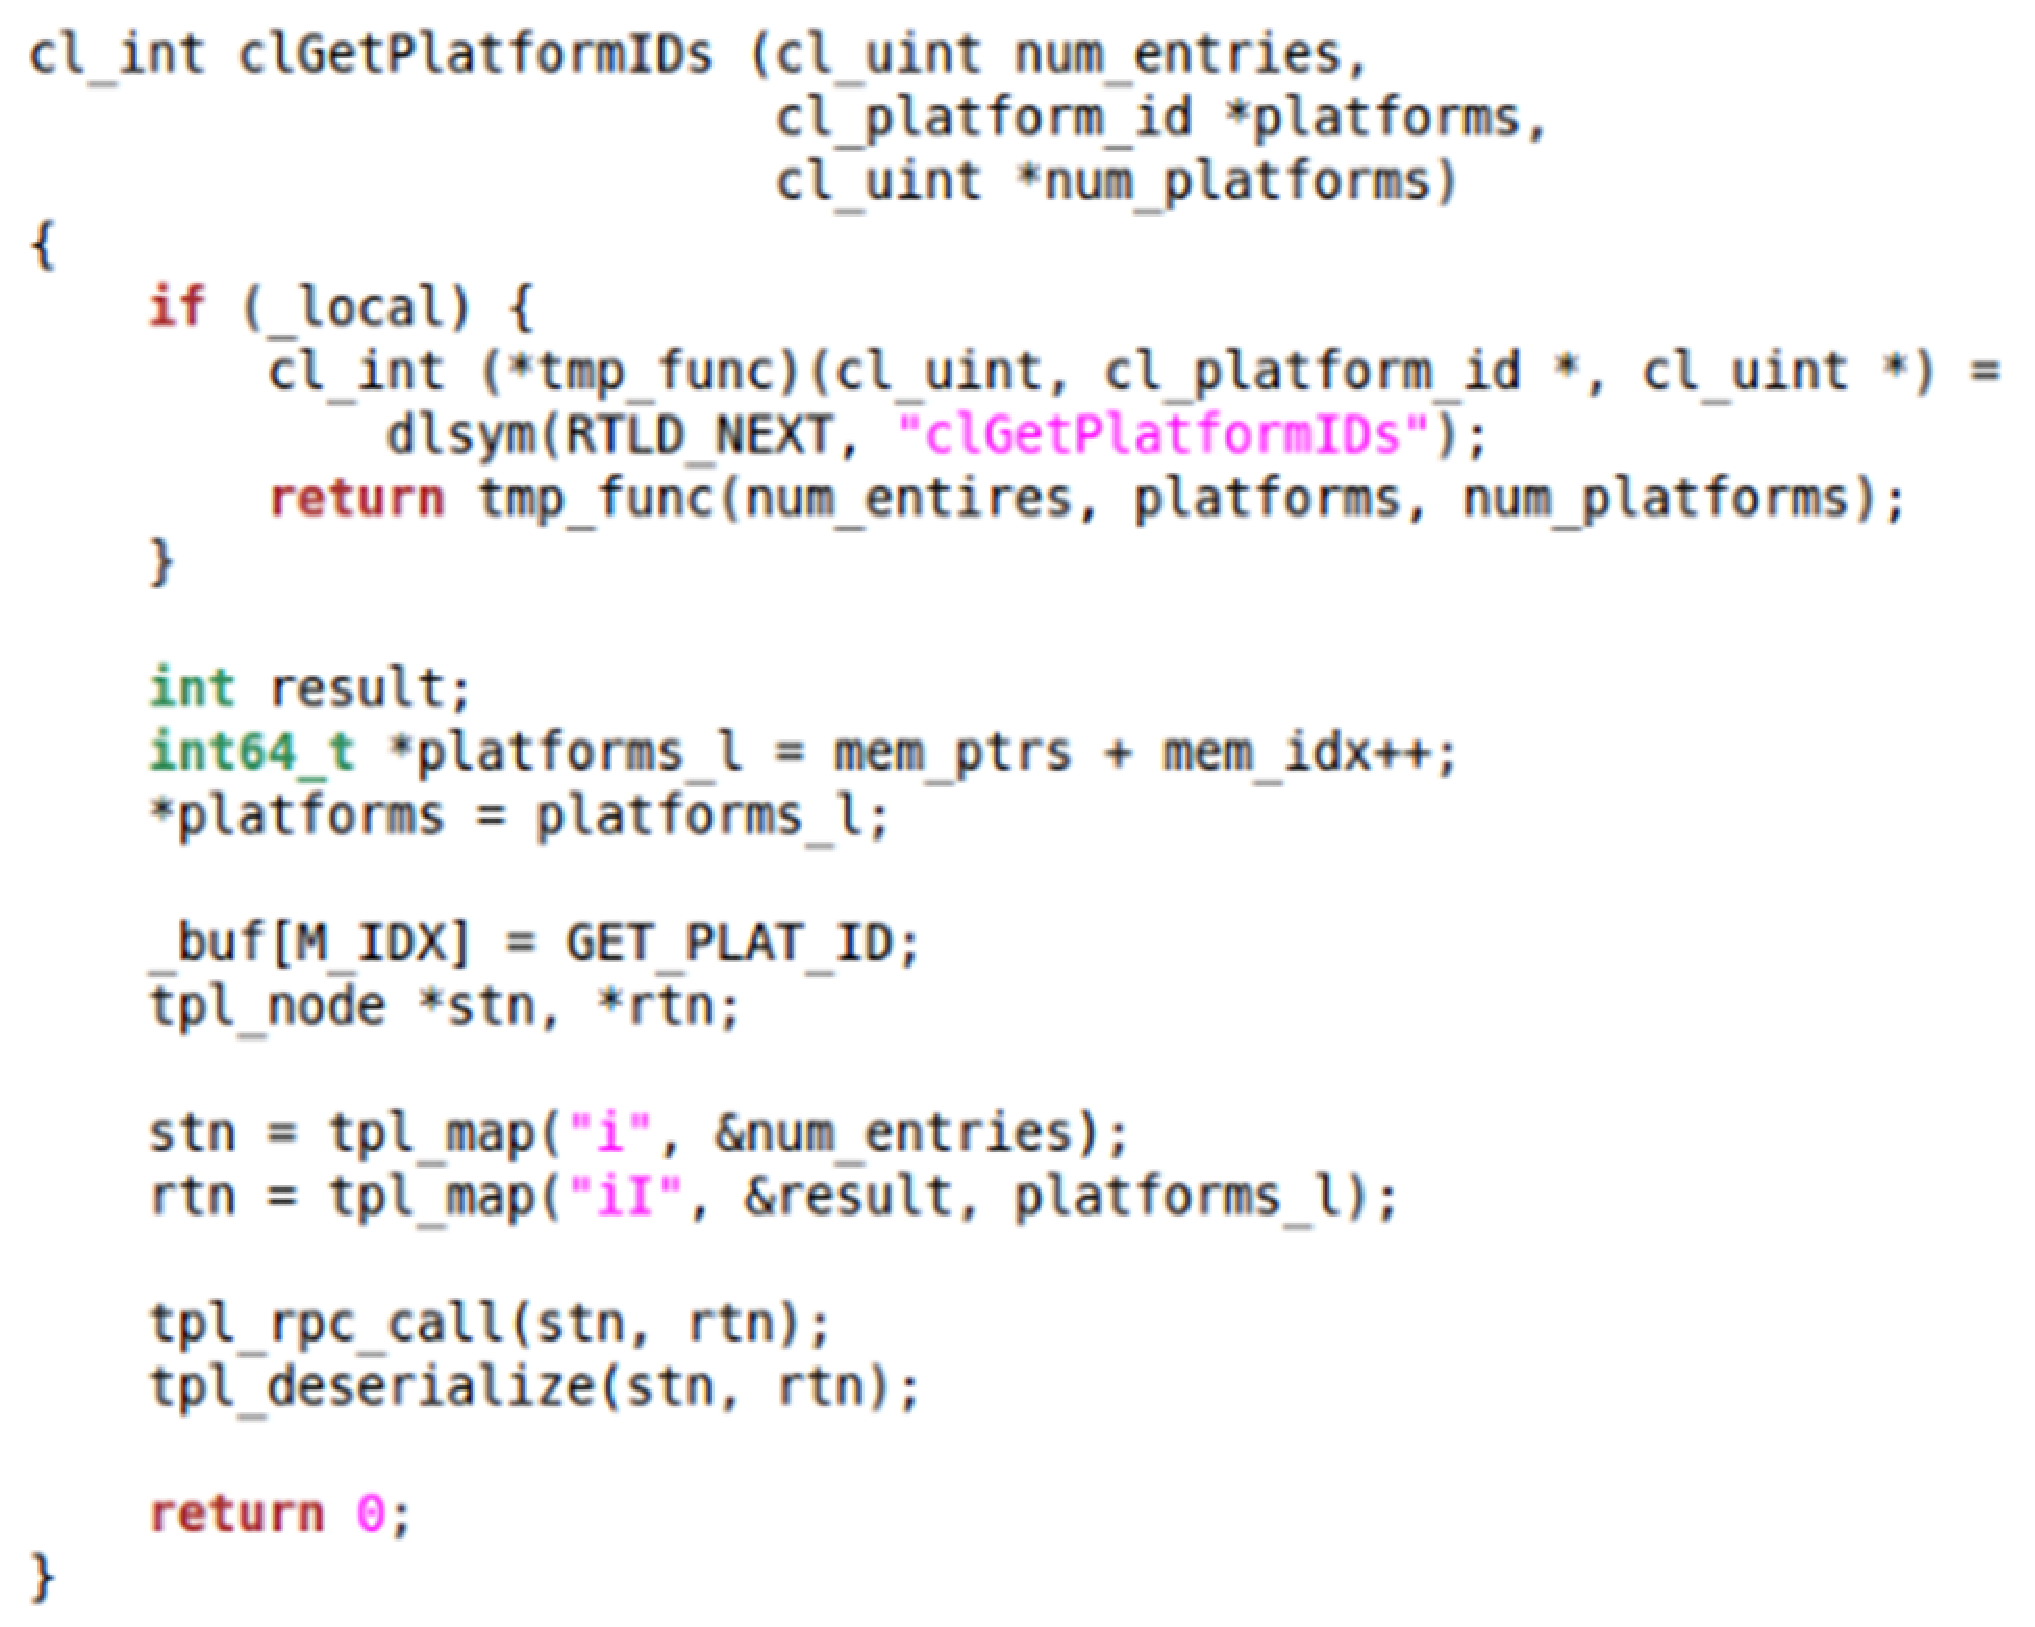
\epsfig{file=figs/code_rpc.eps, width=4.0in}
\caption{Code snippet for tntegration of OpenCL API with RPC}
\label{fig:code_rpc}
\end{figure}
%
The integration of OpenCL API with RPC-based service is realized as a
wrapper library which provides an identical interface to the original
OpenCL API.
%
Figure~\ref{fig:code_rpc} presents the codes snippet for wrapped
OpenCL API, {\it{clGetPlatformIDs}}, which is used to retrieve the
information of a targeted remote resource.
%
In the wrapper library, if a runtime scheduler, which will be described
in section~\ref{offloading:scheduler}, decides to execute the workload
locally, the wrapper library routes these API invocations to the original
local OpenCL library to invoke the corresponding OpenCL API.
%
On the other hand, the wrapper library serializes the API name and
arguments for remote execution, invokes the corresponding remote procedure
call, and sends them to the targeted remote resource over the network.
%
For data serialization, I use the efficient serialization package called
TPL data serialization~\cite{tpl}.
%
TPL can be used to serialize files, memory buffers and file descriptors
so that it is appropriate for use as a file format or inter-process
communication message format.
%

\subsection{Runtime Scheduler}
\label{offloading:scheduler}
%
As previously mentioned, the OpenCL-based remote offloading framework
provides developers with a list of accelerators(both local and remote)
to select as offloading targets.
%
However, some application developers may not want to bother with this
cumbersome task of figuring out which devices would make a good
candidate for local execution versus remote offloading.
%
The proposed framework provides a runtime scheduler which plays a key
role in the framework because it is the module that profiles performance
dynamically at runtime and codifies the policies designed to maximize
energy performance by selectively offloading tasks.\\ 
%
In the current implementation, the runtime scheduler consists of two
main parts: a resource profiler and a decision maker.
%
The default behavior of the resource profiler is to keep track of
network latencies to available remote resources and when the decision
maker requests the target to offload the workload, the profiler
provides the remote resource with lowest latency.
%
Then, the decision maker determines dynamically if the workload should
be offloaded or executed locally.
%
I  will explain the machine learning-based decision making in
section~\ref{chap:scheduler} in detail.\\
%
Currently, the resource profiler is an overly simplistic model by
considering only network latency as a feature for remote resource
selection.
%
Therefore, I plan on supporting a more complex set of conditions to
select the best remote resource.
%
For instance, by periodically recording the network
conditions (i.e. latency and bandwidth) measured at the VPN layer, and
others features such as computing capabilities of remote resources, the
profiler can automatically make the selection for which remote resources
would yield the best performance for a given condition while maximizing
a certain objective function on the utilization for remote resources.\\
%
This utility function-based resource profiler is motivated by my
previous research work on a peer-to-peer self-organizing and
self-managing cluster system based upon network coordinates and utility
function called SOLARE which stands for self-organizing latency-aware
resource ensemble~\cite{solare}. 
%
In the system, a peer-to-peer node periodically monitors the status of
the cluster in which it is currently involved, and whenever the utility
of the cluster is dropped below a threshold, it migrates to another
cluster to maximize the utility value.
%
In order to make use of utility function, I used two features: the
virtual distance to the cluster in artificial network coordinate system
and the number of current members in the cluster.\\
%
By adopting the module of utility function with different features for
utility function (i.e. latency, bandwidth, computing capabilities of
remote resources and so on), I expect that the remote resource profiler
provides more flexible ability of on-demand resource selection. 
%

\subsection{Decentralized Resource Discovery}
\label{offloading:discovery}
%
\begin{figure}
\centering
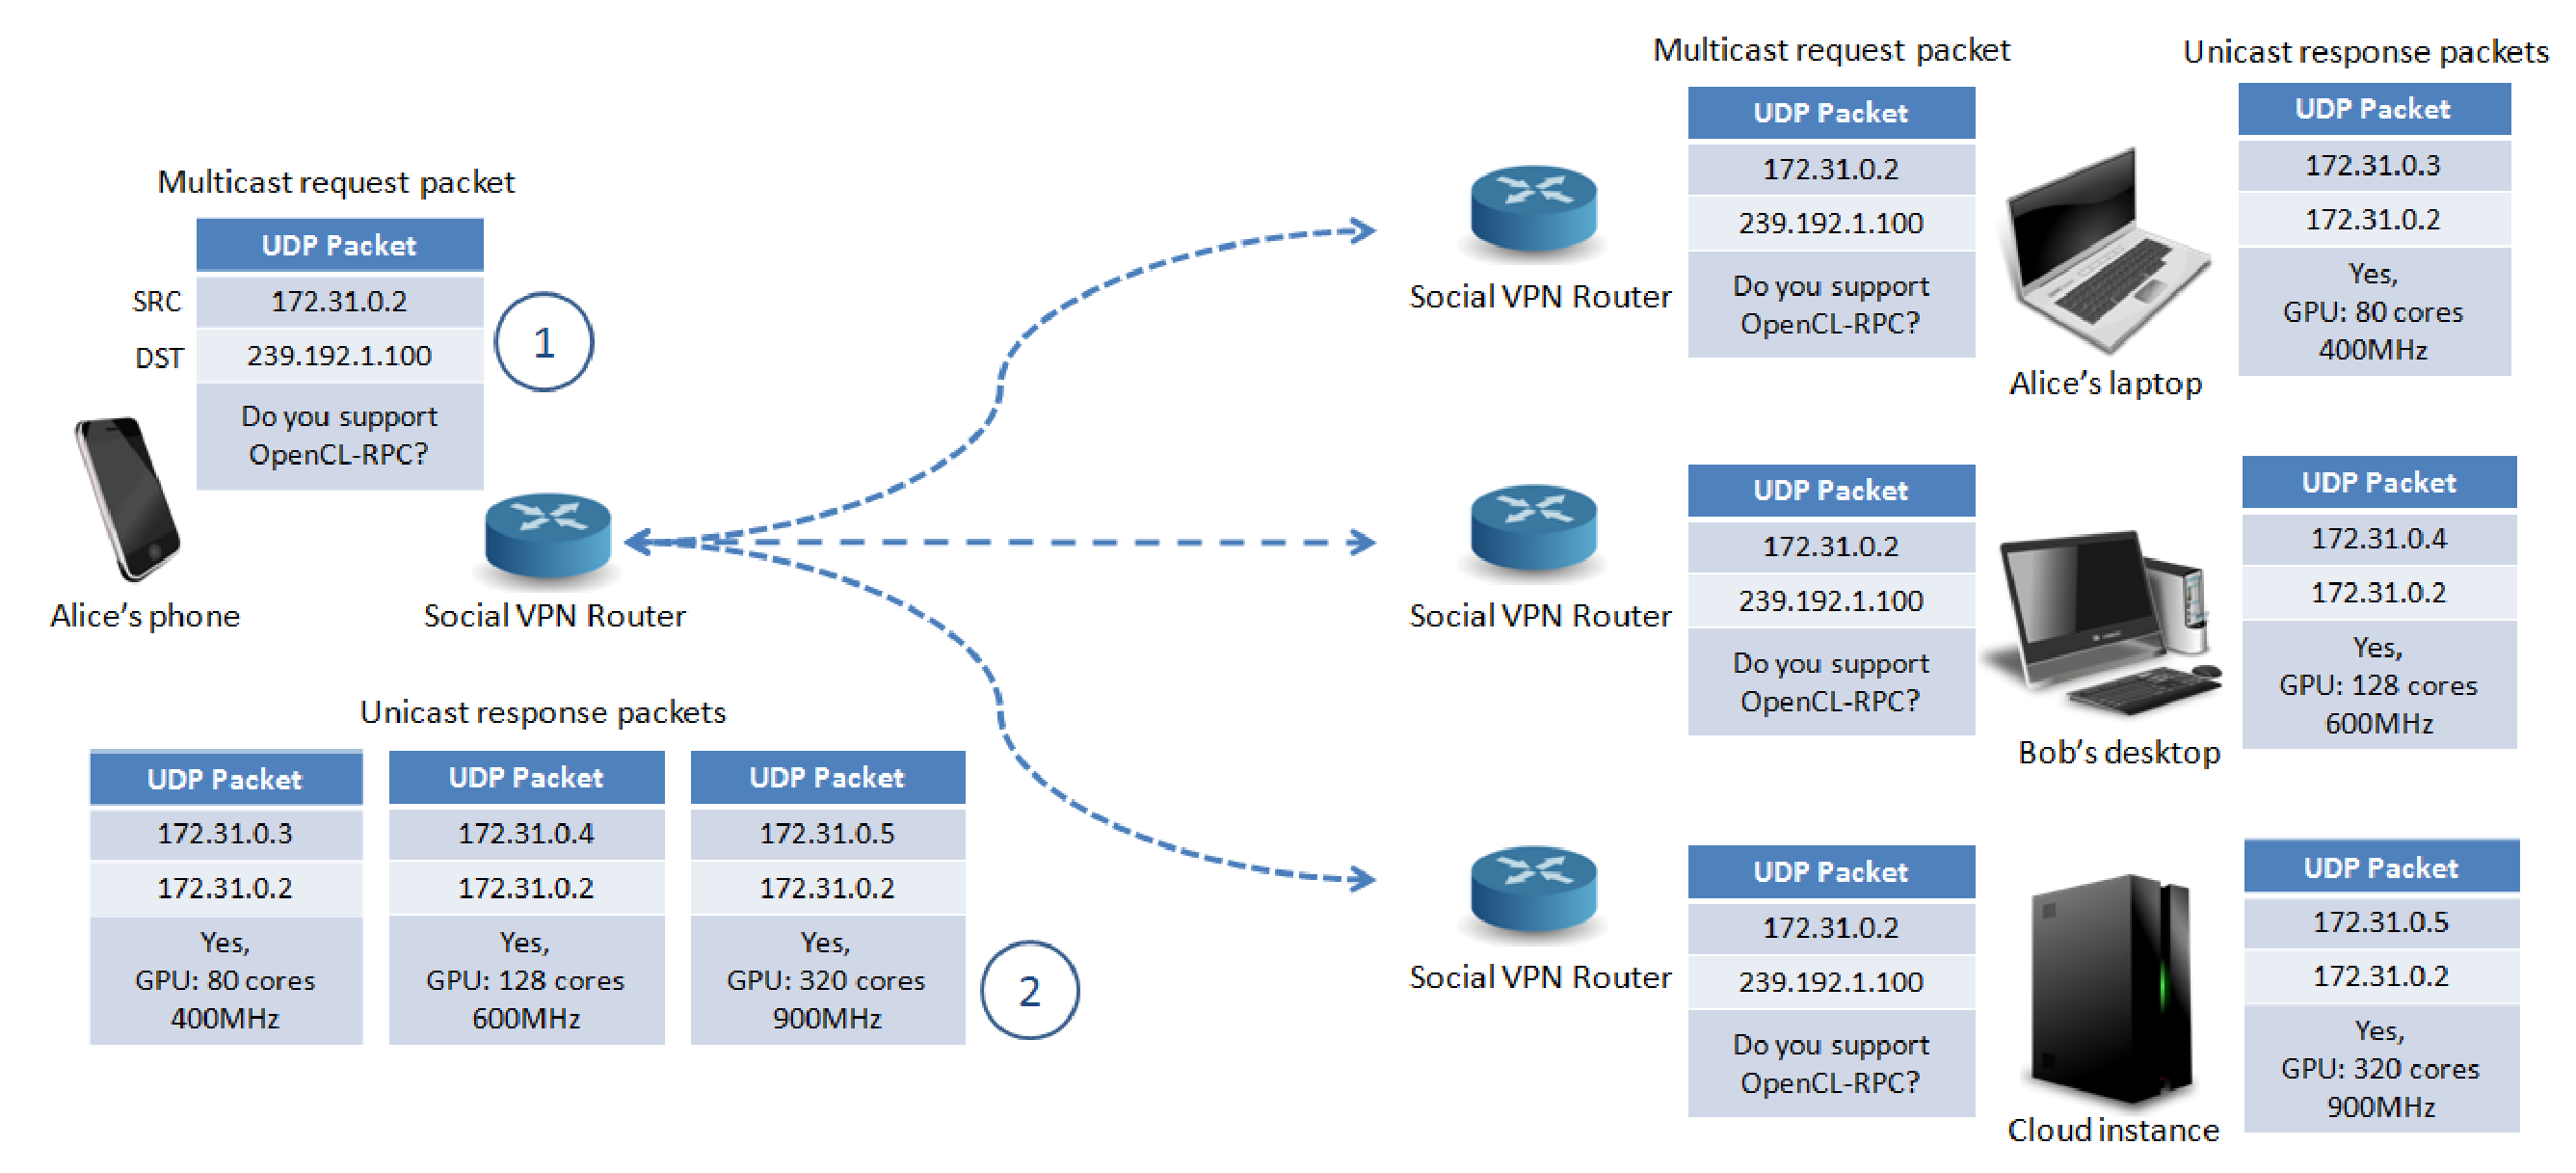
\epsfig{file=figs/discovery.eps, width=6.5in}
\caption{Decentralized resource discovery}
\label{fig:discovery}
\end{figure}
%
Current mobile offloading solutions rely on a centralized service ot
provide the resource discovery capability.
%
A key differentiation of my approach is the decentralized IP
multicast-based remote resource discovery subsystem.
%
A challenge with IP multicast resource discovery mechanism is that the
vast majority of ISPs prevent multicast traffic from traversing their
network.
%
I sidestep this issue with network virtualization through SocialVPN.
%
Because the OpenCL-based remote offloading system is deployed on top of
SocialVPN which enables IP multicasting over the Internet, it is
possible to leverage existing LAN-based service discovery techniques for
wide area environment as well as local area environment.
%
The way that the decentralized remote resource discovery mechanism works
is illustrated in Figure~\ref{fig:discovery}.
%
The client periodically polls the network for eligible remote resources
by sending a UDP datagram to the multicast IP address.
%
The SocialVPN router distributes the IP packet to every remote resource
in the private network.
%
The RPC-based service described in section~\ref{offloading:rpc} has a
UDP listening thread that waits for resource discovery request and
responds to the request with its computing capabilities using the
requestor's unicast IP address.
%
The requester waits for a certain amount of time and accumulates all the
replies that it receives within that time window.
%
The requestor records their latency, bandwidth, and processing
capabilities and provides them to the scheduler.
%
The scheduler then determines which remote resource will provide the
best performance and selects that resource as the targeted candidate.
%
\subsection{Trusted Communication via VPN}
%
\label{offloading:vpn}
The virtual networking component addresses two key challenges of remote
workload offloading -- privacy and peer discovery -- while supporting
unmodified TCP/IP applications to offload computation to remote
computing resources.
%
In order to augment the mobile platform's computing capabilities, it is
important to find trusted resources that are not only in the same local
area network, but also geographically-dispersed peers, and to do so
dynamically an transparently to the mobile user's application.
%
While many VPN tunneling techniques would be applicable (e.g.
OpenVPN~\cite{openvpn}, Hamachi~\cite{hamachi}), the approach chosen in
the prototype is SocialVPN~\cite{socialvpn}, due to its ability to
autonomously create and manage VPN links to social peers, and its
support for tunneling IP multicast and discovery.
%
SocialVPN is a decentralized, self-configuring VPN based on online
social networking services such as XMPP and a public-key based security
model where certificates are exchanged and used to setup VPN links
automatically using online social network APIs.
%
SocialVPN ensures that friends anywhere on the Internet appear to be on
the same virtual LAN and end-to-end encrypted peer-to-peer tunnels are
abstracted as virtual IP links among friends.
%
SocialVPN  autonomously and continuously takes care of discovering and
exchanging public-key VPN certificates with social peers through online
social network infrastructures, handling the assignment and mapping of
virtual private IP addresses to devices, creating security associations
among peers, and capturing/routing IP packets for secure end-to-end
tunneling leveraging a peer-to-peer overlay.
%
By leveraging SocialVPN as a trusted peer-to-peer messaging substrate,
it is possible to use the Berkeley sockets networking interface to
offload the mobile workloads without any direct linking to SocialVPn
itself.
%
Most peer-to-peer systems require integration with a peer-to-peer
library as well as a learning curve for learning curve for learning its
API.
%
Because SocialVPN provides virtual private IP addresses to friends
instead of P2P addresses, it supports unmodified applications.
%

\section{Evaluation}
\label{offloading:evaluation}
%
In this section, I evaluate the implementation of the OpenCL-based
remote offloading framework for mobile platforms in terms of the
performance and energy consumption for mobile devices through real
deployment over local and wide area environments.
%
Firstly, I quantitatively analyze the overhead of the proposed resource
discovery mechanism in terms of energy consumption as a function of
number of remote resources.
%
Next, I will demonstrate the ability of the decentralized resource
discovery mechanism to dynamically discover remote resources under the
situation where the client offloads the workload iteratively to the best
resource with respect to the network latency while a few remote
resources occasionally join or leave the private network.
%
Also, I examine the overhead of adopting SocialVPN to the secure
communication between the client and the remote resource since SocialVPN
utilizes its own encryption and IP tunneling.
%
\subsection{Experimental Setup}
\label{offloading:setup}
In order to evaluate our remote offloading framework under a variety of
possible use case scenarios, I setup the experiments using various
hardware and network configurations.
%
First of all, for the mobile client, I utilized an Android table,
Samsung GalaxyTab 10.1 equipped with 1Ghz dual-core processor and 1GB
RAM, and running Android 3.1.
%
For the SocialVPN-connected remote resources, I utilized a workstation
with Intel 3.0Ghz Core2 Duo processor and 8GB memory installed with
Linux OS.
%
In addition, I used Amazon EC2 GPU cluster resource~\cite{amazonec2} and
FutureGrid virtual instances~\cite{futuregrid} for the remote resources which have
different computing capabilities and network performance.\\
%
For offloaded OpenCL workloads, I utilized OpenCL SDK code samples
provided by AMD SDK~\cite{amd} and NVIDIA~\cite{nvidia} such as
Sobelfilter, matrix multiplication, N-body physics,
and hidden Markov model\footnote{I will describe more details about
OpenCL workloads that I chose for the experiments in
Section~\ref{chap:character}}.
%
Also, I emulate different wide area network conditions between the
client and the remote resource by controlling the network latency using
Traffic Control(TC)~\cite{tc}.
%
TC is a network tool which  provides functionality to control network
traffic by prioritizing network resources and using concepts of traffic
classification, queue disciplines and quality of service.
%
To profile energy consumption of the mobile device, I used
PowerTutor~\cite{powertutor} which is an application for the variants of
Android devices that displays the power consumed by major components
such as CPU, network interface, LCD display, and GPS receiver.
% 
\subsection{Overhead of Resource Discovery}
\label{offloading:overhead_discovery}
%
\begin{figure}
\centering
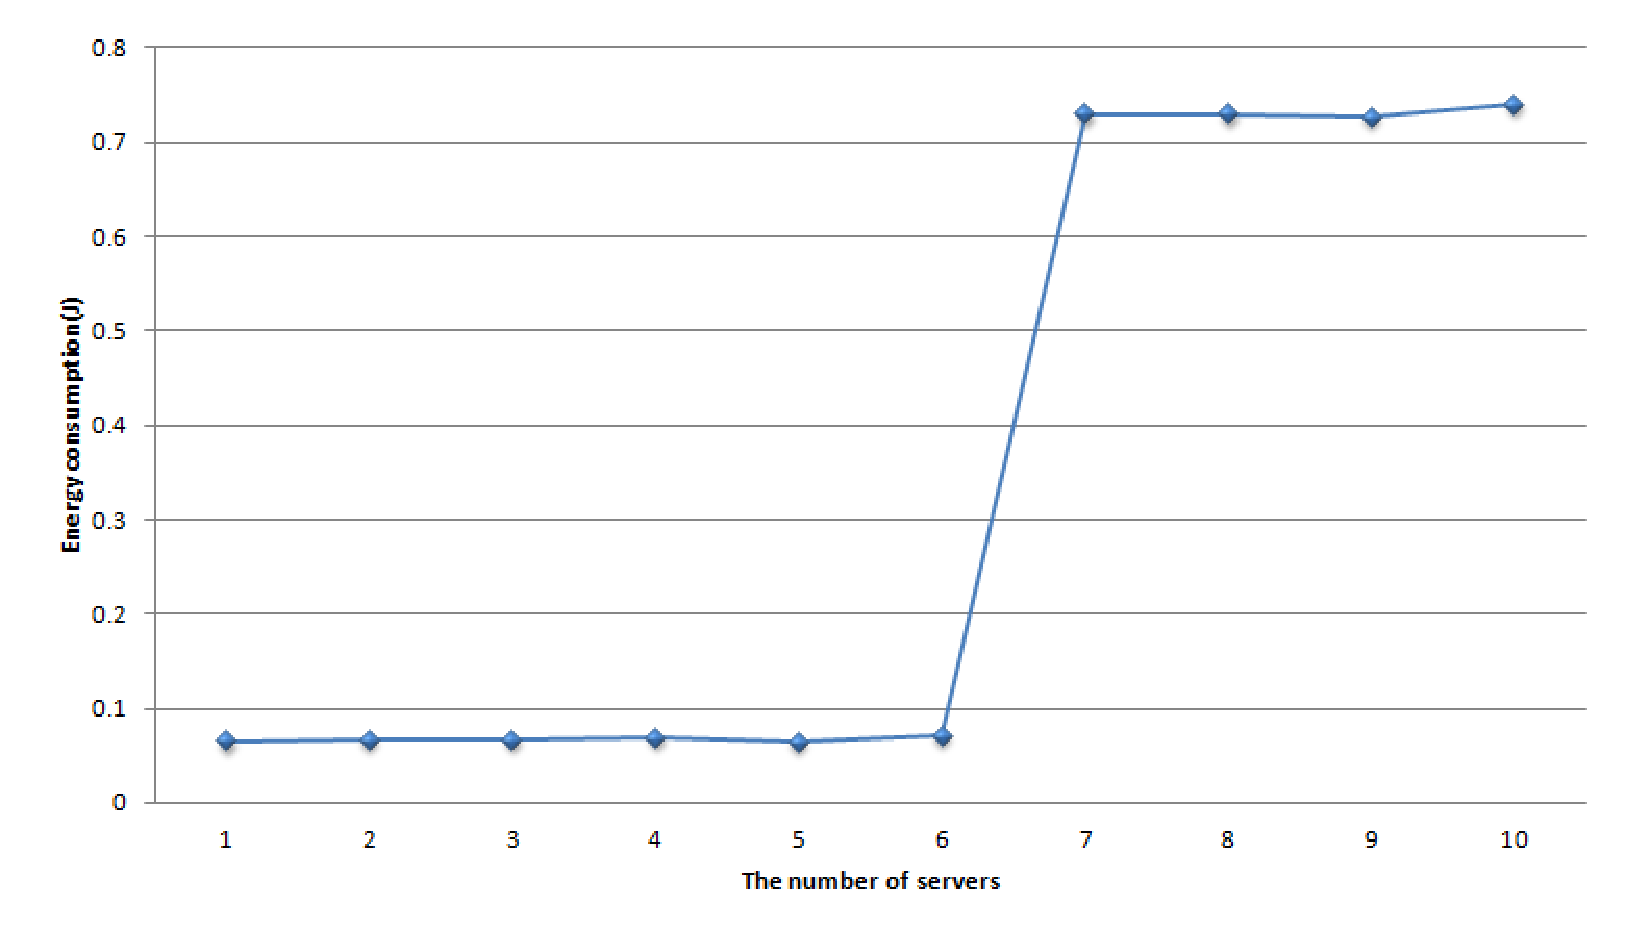
\epsfig{file=figs/energy_discovery.eps, width=4.5in}
\caption{Energy consumption for resource discovery mechanism}
\label{fig:energy_discovery}
\end{figure}
%
A novelty of this work is to allow the users to dynamically and
transparently discovery the remote resources through IP multicasting on
top of SocialVPN.
%
However, as the number of remote resources increases, the burden that
the mobile device has to handle also increases as well.
%
For that reason, it is essential to quantify the costs of the resource
discovery mechanism in terms of energy consumption of the mobile
devices.
%
I have conducted a WAN experiment in which 10 remote resources bound to
SocialVPN overlay are deployed in virtual machines at
FutureGrid~\cite{futuregrid} resources at University of Chicago,
University of California San Diego, and University of Texas, while a
client located at University of Florida requests the resource discovery.
%
Figure~\ref{fig:energy_discovery} shows energy consumption while the mobile
device performs the resource discovery for the given number of
resources.
%
As shown in Figure~\ref{fig:energy_discovery}, up to six resources,
energy consumption of the resource discovery does not vary
significantly, at less than 0.1J, regardless of the number of the
resources.
%
However, from seven resources onward, energy consumption jumps up to
0.7J.
%
This is because a typical Wi-Fi networking device can tolerate the
number of packets to multicast resource request messages and to receive
the replies from up to six resources without entering into high power
mode.
%
However, the number of packets with seven resources crosses this
threshold pushing the Wi-Fi device into high power mode and resulting in
more energy consumption.
%
It is worth noting that the overhead of energy consumption from resource
discovery mechanism depends on the interval of resource discovery which
means the trade-off between energy consumption and the accuracy of the
network characteristics of available remote resources.
%
In current setting, the resource discovery is repeated every 60 seconds
which means only 4.6\% of the overhead compared with when matrix
multiplication is executed locally consuming 15J of energy for 60
seconds(Section~\ref{character:energy}).
%
\subsection{Dynamic Resource Discovery}
\label{offloading:dynamic}
%
\begin{figure}
\centering
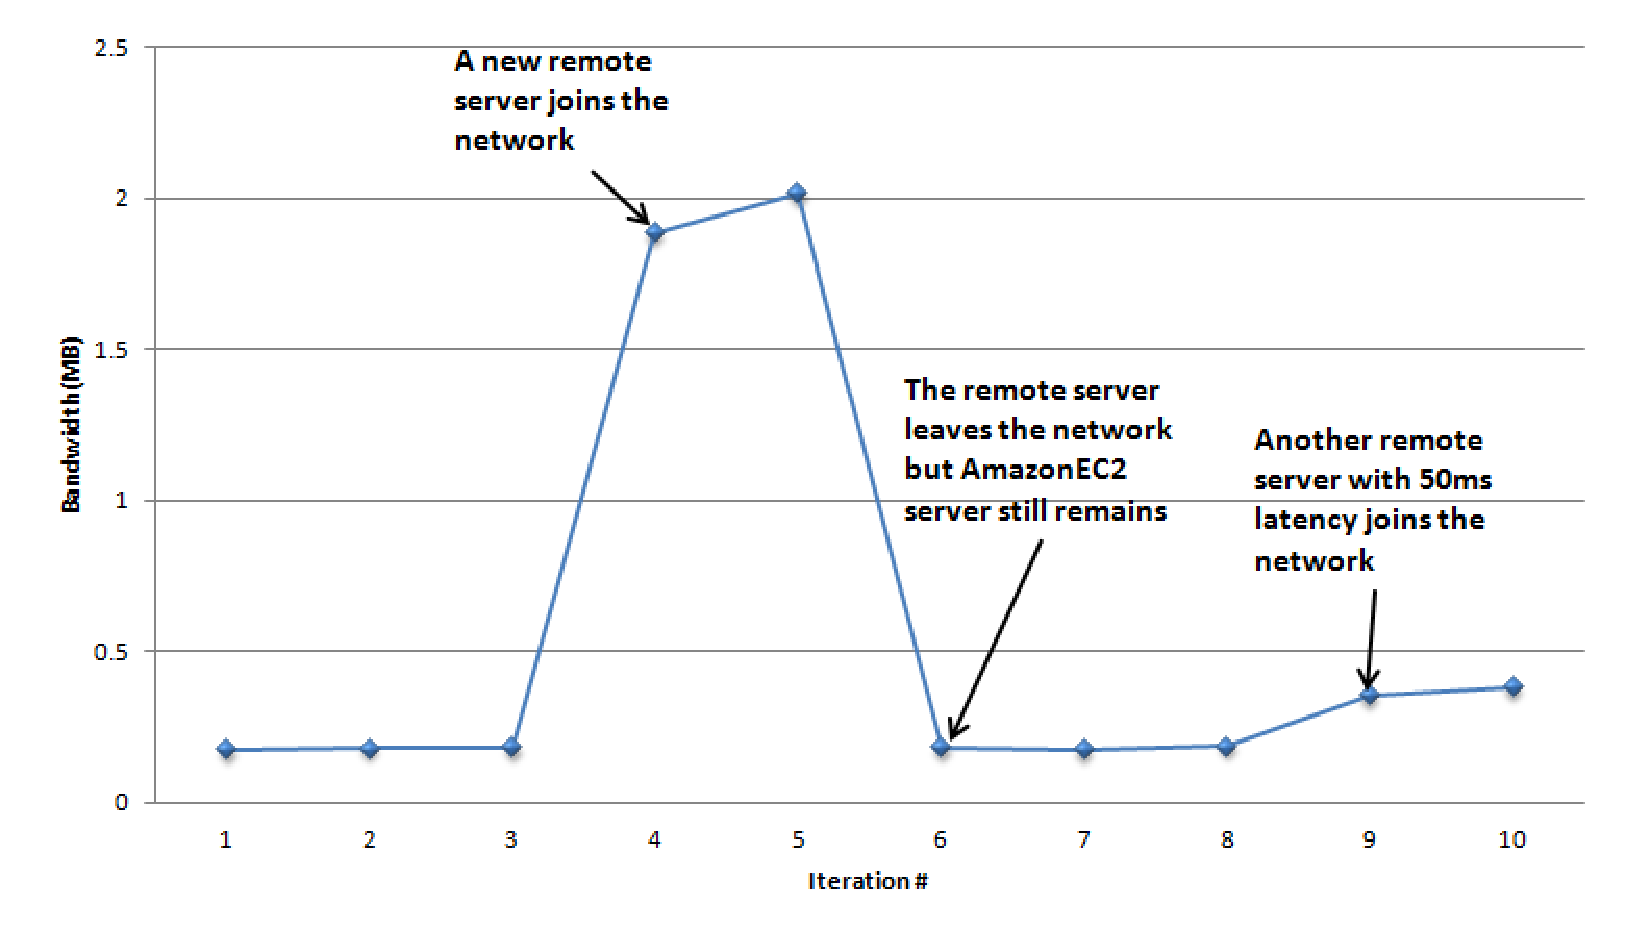
\epsfig{file=figs/dynamic_discovery1.eps, width=4.5in}
\caption{Bandwidth measurement}
\label{fig:dynamic_discovery1}
\end{figure}
%
\begin{figure}
\centering
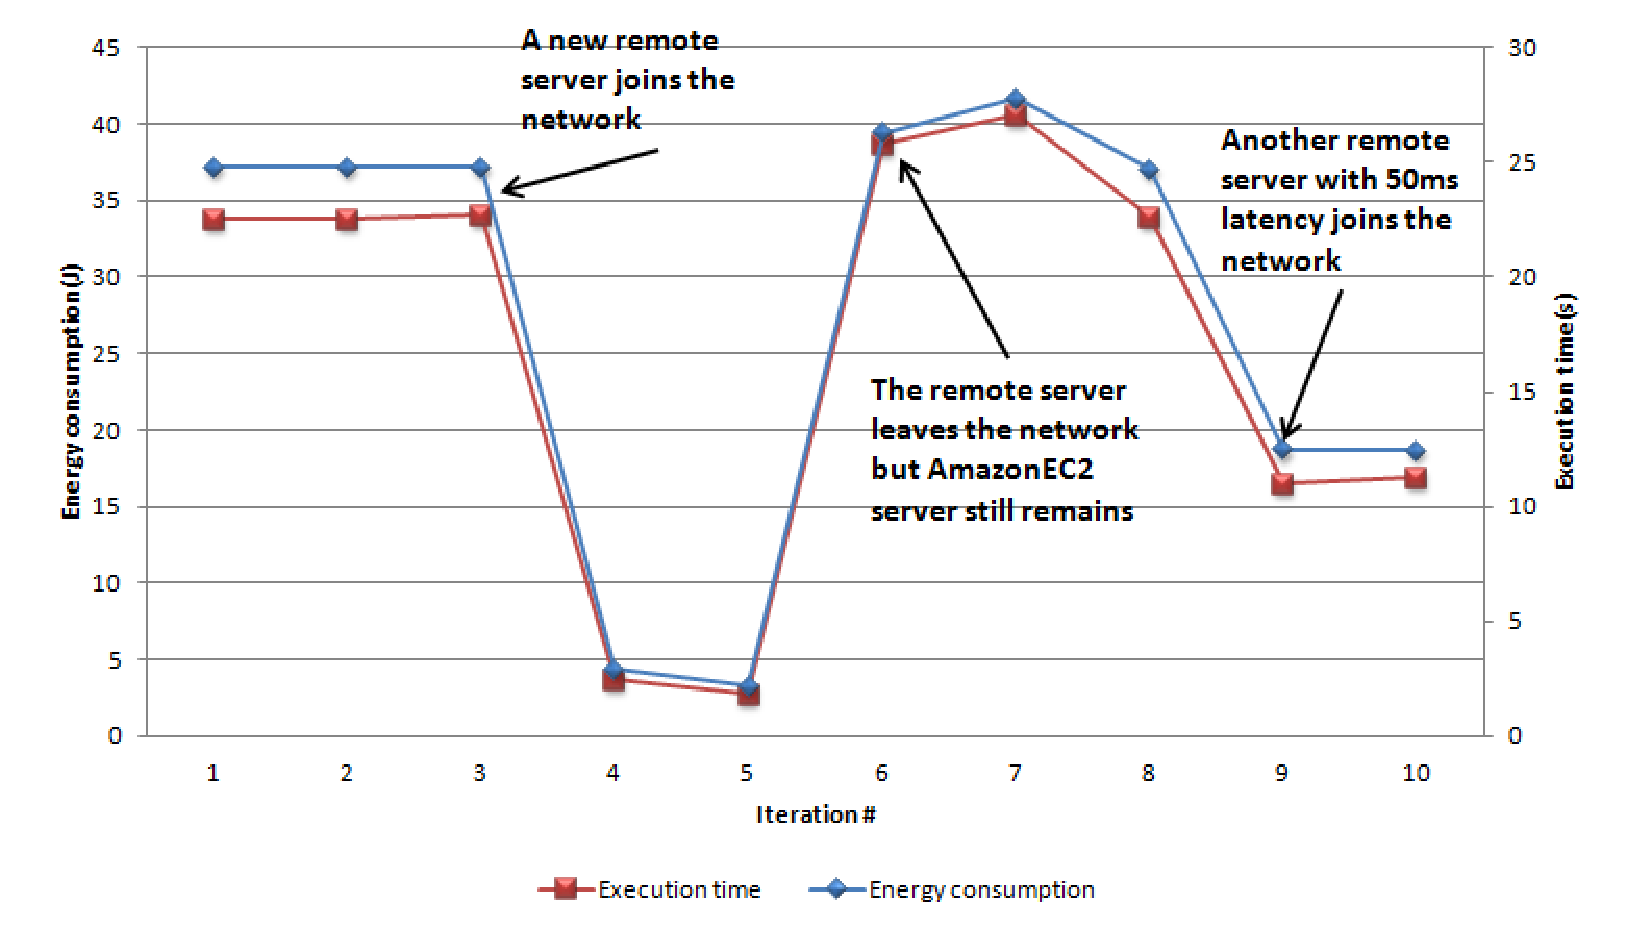
\epsfig{file=figs/dynamic_discovery2.eps, width=4.5in}
\caption{Performance measurement of remote offloading}
\label{fig:dynamic_discovery2}
\end{figure}
%
In this section, I demonstrate the ability to dynamically discover the
remote resources while the resources join or leave the networks and the
client offloads hidden Markov model to the remote resource.
%
For this, I designed a simple experiment in which the client offloads
the workload iteratively to the best resource with respect to the
network latency while a few servers occasionally join or leave the
network.\\
%
Firstly, when the client starts executing the workload, it has only one
available remote resource launched at Amazon EC2 GPU cluster and
offloads the workloads until a better remote resource is available.
%
At the fourth iteration, a new remote resource, which has less than 10ms
latency, joins the network.
%
As a result, the client connects to the new remote resource and switches
offloading to the new resource.
%
And then, at the sixth iteration, the remote server leaves the network
but Amazon EC2 resource still remains, so the client offloads the
workload to Amazon EC2 resource again.
%
Finally, another new remote resource with 50ms latency joins and the
client contacts to that resource.
%
Figure~\ref{fig:dynamic_discovery1} and ~\ref{fig:dynamic_discovery2} show the
available bandwidth to the best resource and the performance of remote
offloading respectively while resources join or leave the private
network.
%
\subsection{Overhead of SocialVPN}
\label{offloading:overhead_socialvpn}
%
\begin{figure}
\centering
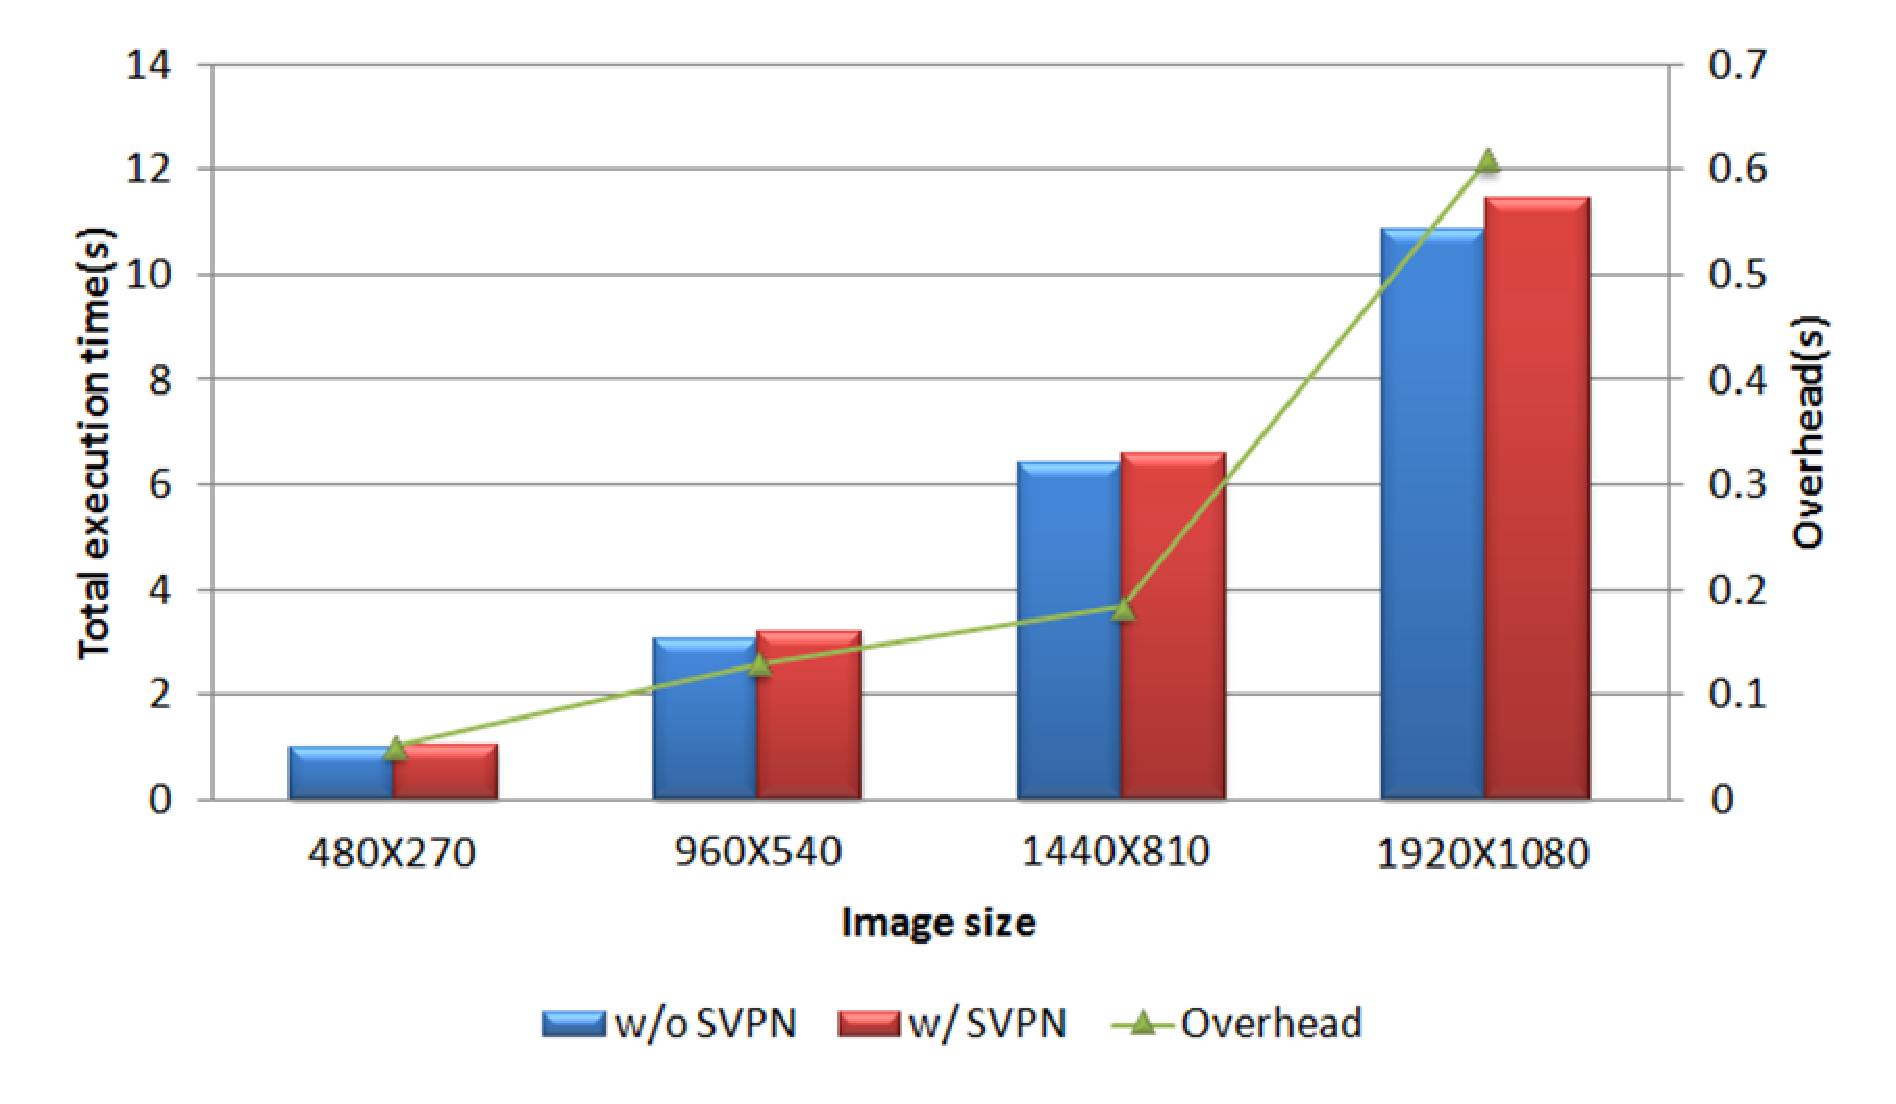
\epsfig{file=figs/overhead_socialvpn1.eps, width=4.5in}
\caption{Overhead of SocialVPN in terms of execution time}
\label{fig:overhead_socialvpn1}
\end{figure}
%
\begin{figure}
\centering
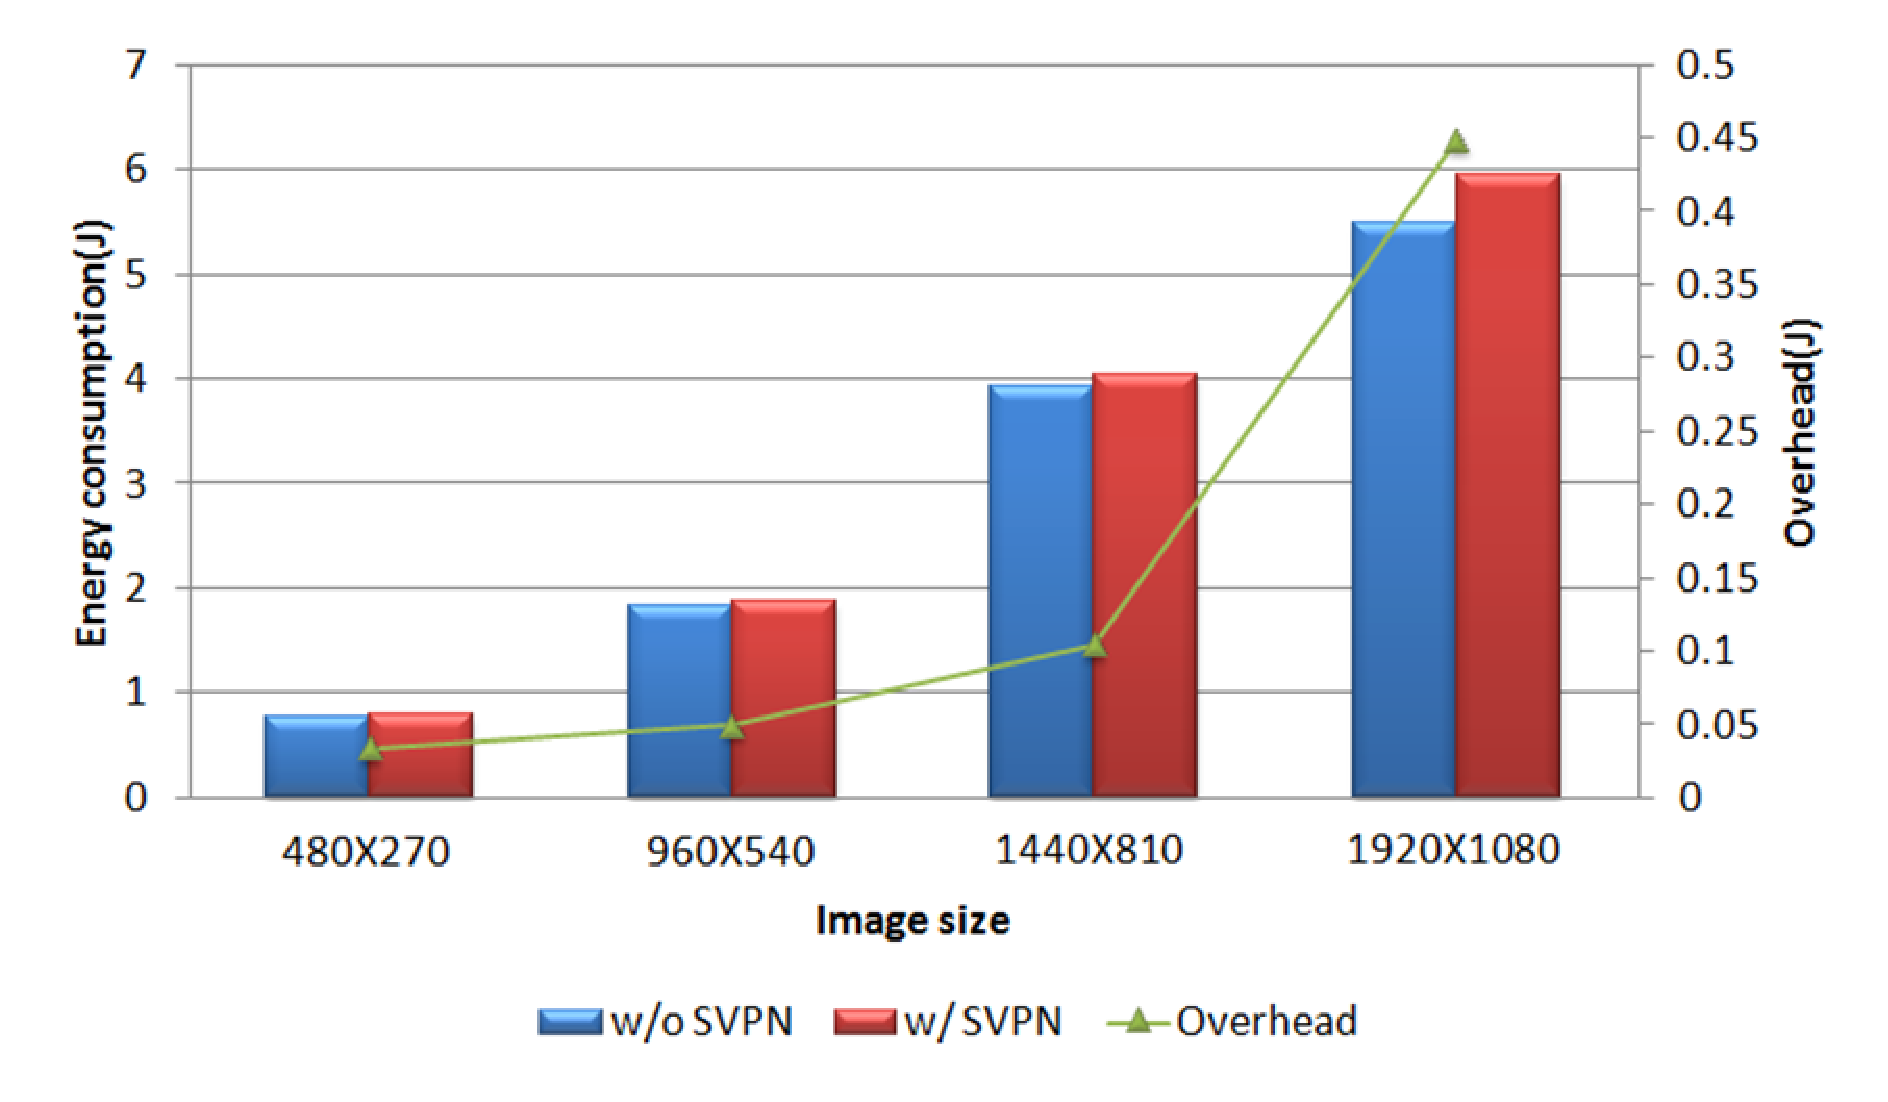
\epsfig{file=figs/overhead_socialvpn2.eps, width=4.5in}
\caption{Overhead of SocialVPN in terms of energy consumption}
\label{fig:overhead_socialvpn2}
\end{figure}
%
In the OpenCL-based remote offloading framework, SocialVPN enables
mobile devices and remote resources to securely communicate.
%
This incurs overheads due to encryption and tunneling.
%
In this section, I investigate the overhead of SocialVPN with respect to
the performance and energy consumption.
%
In order to measure the overhead of SocialVPN, I have conducted the
experiments in local area networks in which the client offloads OpenCL
workloads to the remote resource both with and without SocialVPN.
%
I do not consider the wide area network experiments for this comparison
because the resource discovery mechanism without SocialVPN is not viable
in wide area networks due to hindering of multicast by ISPs.\\
%
Figure~\ref{fig:overhead_socialvpn1} and ~\ref{fig:overhead_socialvpn2}
show the offloading execution time and energy consumption with and
without SocialVPN, respectively.
%
Even though I carried out the experiments using all of the workloads
I implemented, I only present the results from Sobelfilter because
other workloads also show the similar trend as Sobelfilter.
%
As shown in Figure~\ref{fig:overhead_socialvpn1}, as the image size
increases, the execution time and energy consumption also increase.
%
In the case of 480$\times$270 of image size, for instance, offloading with
SocialVPN takes 0.05s more than without SocialVPN while it takes 0.6s
more to offload 1920$\times$1080 of image size which means that the
overhead ranges from 2.8\% to 5.6\%.
%
In Figure~\ref{fig:overhead_socialvpn2}, I also observed the overhead
ranging from 2.6\% to 8.1\% in terms of energy consumption.
%
SocialVPN appends 80 bytes of an additional header to every packet to
tunnel regular TCP/IP packets where the default MTU(Maximum Transmission
Unit) for the experimental setup is 1,480 bytes.
%
For that reason, I approximately calculated about 6\% of the overhead
coming from SocialVPN.
%

\section{Summary} 
\label{offloading:summary}
In this section, I presented the OpenCL-based remote offloading
framework designed specifically for mobile cloud computing where OpenCL
workloads can be exported from a mobile device (i.e. an Android device)
to trusted remote resource (i.e. friend's desktop or family's laptop) or
even to the cloud resource (i.e. an Amazon EC2 instance with GPU
access).
%
The proposed remote offloading system consists of the following main
components: 1) a customized RPC-based service with optimizations for
network tasking and data marshalling, 2) a resource discovery mechanism
which selects the remote resource with the lowest latency, and 3) a
virtual private networking layer which provides transparent network
encryption without any modification at the application layer.\\
%
First of all, the prototype of the proposed remote offloading framework is implemented
as a wrapper library around the OpenCL API while allowing transparent
integration of the OpenCL API with RPC-based service without any code
modification.
%
Also, the IP multicast-based resource discovery mechanism makes it possible
for the mobile device to dynamically discover remote resources during
runtime and to utilize the computing capabilities of remote resources.
%
Furthermore, the proposed approach supports accessing resources beyond
the local private network, broadening the accessibility to trusted
remote resources across the Internet and the cloud.
%
This is accomplished by utilizing a social peer-to-peer virtual private
network, SocialVPN and creating a Social Area Network in which only
trusted social peers' computing resources are involved.\\
%
The evaluation showed that the use of SocialVPN resulted in a reasonably
acceptable overhead while guaranteeing secure connections and data
privacy.
%
Also, I demonstrated the ability to dynamically discover remote
resources while remote resources join or leave the network.
%
 
